\chapter{Theorie}
\section{Das Spiel Tic-Tac-Toe}

Tic-Tac-Toe ist ein sehr altes, klassisches Strategiespiel, welches von zwei Personen gespielt wird. Eine Person
spielt hierbei das Symbol Kreuz und eine andere Person das Symbol Kreis. Das Spielfeld von Tic-Tac-Toe besteht aus
neun Feldern, in denen die entsprechenden Symbole verteilt werden können. Jeder Spieler setzt hierzu abwechselnd sein
Symbol in eines der neun Felder. Es ist nicht möglich ein bestehendes Symbol zu überschreiben oder mehrere Symbole in
ein Feld zu zeichnen. Der Anfang einer Runde Tic-Tac-Toe kann beispielsweise wie folgt aussehen:
\begin{figure}[H]
    \centering
    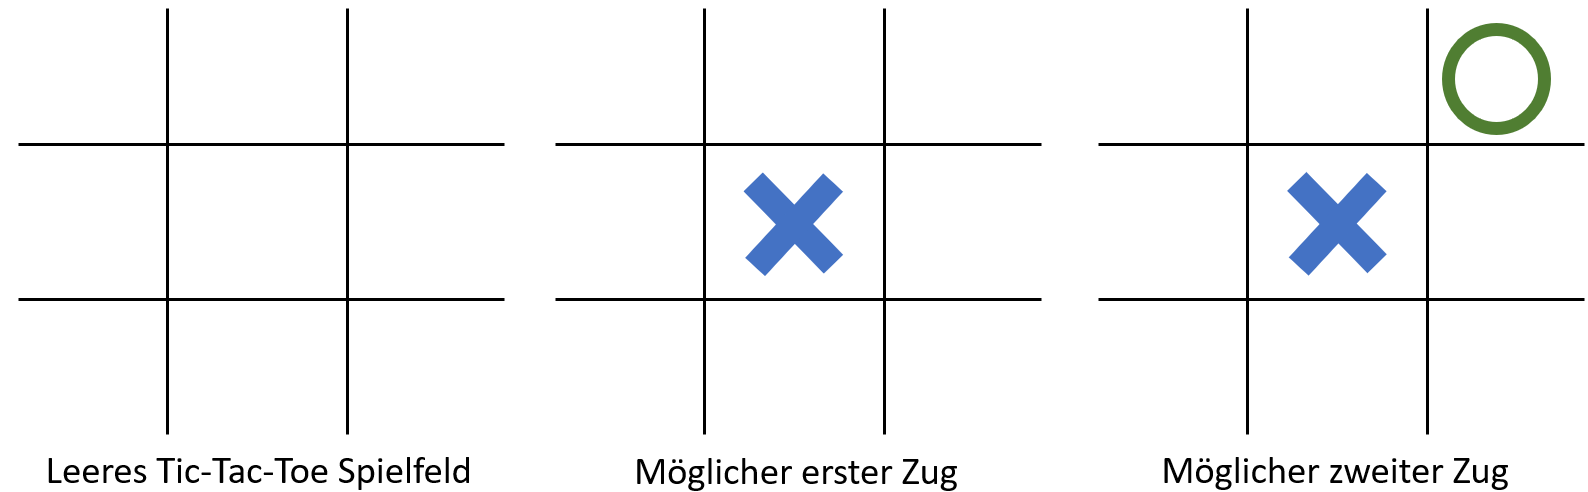
\includegraphics[scale=0.25]{img/tictactoe_start.png}
    \caption[Möglicher Anfang eines Tic-Tac-Toe Spiels]{Möglicher Anfang eines Tic-Tac-Toe Spiels (eigene Anfertigung)}
    \label{fig:tictactoestates}
\end{figure}
Im ersten Teil des Bildes erkennt man die neun leeren Felder des Spielfeldes. Im zweiten Teil des Bildes fängt der erste
Spieler damit an, sein erstes Kreuz in die Mitte des Spielfeldes zu setzen. Der zweite Spieler ist nun am Zug und setzt
im dritten Teil des Bildes seinen Kreis in die obere rechte Ecke des Spielfeldes. Als Nächstes wäre Spieler eins wieder an
der Reihe und dürfte sein nächstes Kreuz setzen. Ziel des Spiels ist es, drei gleiche Symbole in einer Reihe, Spalte oder
Diagonale zu haben. Die folgende Abbildung soll dieses Verfahren nochmal genauer erläutern:
\begin{figure}[H]
    \centering
    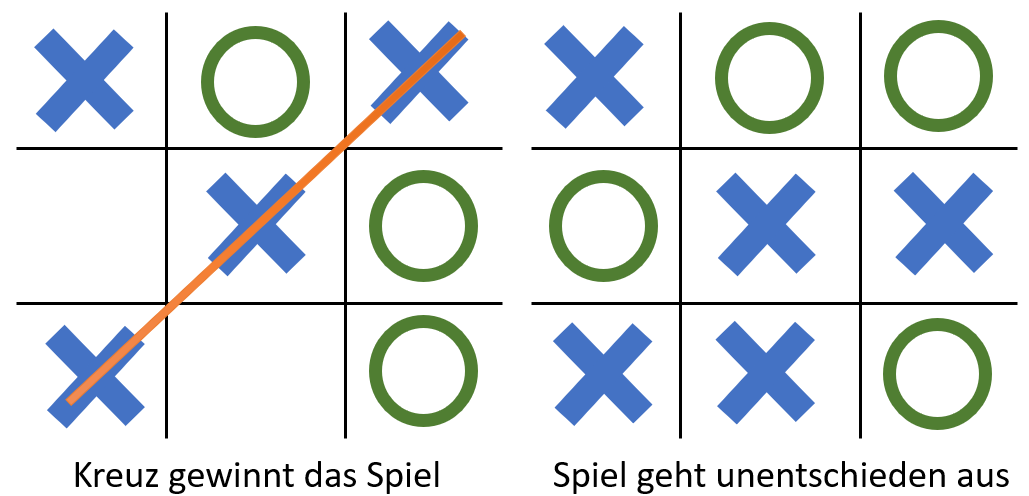
\includegraphics[scale=0.25]{img/tictactoe_endings.png} 
    \caption[Mögliches Ende eines Tic-Tac-Toe Spiels]{Mögliches Ende eines Tic-Tac-Toe Spiels (eigene Anfertigung)}
\end{figure}
Im ersten Teil der Abbildung ist zu sehen, wie der Spieler mit dem Kreuzsymbol drei Kreuze auf einer Diagonale unterbringen
konnte. In diesem Fall ist die Runde beendet und dieser Spieler hat die Runde gewonnen. Ob das Spiel über drei Symbole in einer
Reihe, Spalte oder Diagonale gewonnen wird, ist nicht relevant. Ebenfalls spielt es keine Rolle, in welcher Reihenfolge die 
Symbole gesetzt wurden. Im zweiten Teil des Bildes zeigt sich ein weiteres mögliches Ende für eine Runde Tic-Tac-Toe. Bei diesem
Ende ist das komplette Spielfeld ausgefüllt und es ergeben sich keine drei Symbole in einer Reihe, Spalte oder Diagonale. 
Entsprechend ist die Runde unentschieden ausgegangen.

\section{Der Minimax-Algorithmus}
\label{chap:minimax}
Nachdem das Spiel Tic-Tac-Toe erklärt wurde, soll nun mit Hilfe des Minimax Algorithmus eine künstliche Intelligenz 
entwickelt werden, die in einem Spiel gegen einen menschlichen Spieler immer einen optimalen Zug ausführt. Der Minimax 
Algorithmus baut dabei auf der Funktion \code{value} auf, die wie folgt definiert ist:

\[value: States \times Players \rightarrow \{-1,0,1\}\]

Die Rückgabewerte symbolisieren dabei den worst case Ausgang eines Zuges:

\begin{itemize}
    \item -1 bedeutet, dass der Spieler bei diesem Spielzug im schlechtesten Fall verliert
    \item 0 bedeutet, dass im schlechtesten Fall ein Unentschieden erzielt werden kann
    \item 1 bedeutet, dass mit der Wahl dieses Spielzuges ein Sieg erzielt wird
\end{itemize}

Die Funktion berechnet alle möglichen Folgezüge für das übergebene Spielfeld. Sobald eine Spielsituation 
erreicht wurde, bei der das Spiel entweder von einem Spieler gewonnen wurde oder keine weiteren Spielsteine 
mehr gesetzt werden können, wird die Funktion \code{utility} aufgerufen. Diese vergleicht den Spielzustand 
mit allen möglichen Endzuständen und gibt gegebenenfalls den Gewinner oder Unentschieden zurück. Da der Spieler 
nach jedem Zug wechselt, wird immer abwechselnd der höchste Wert bzw. der niedrigste Wert für den nächsten Zug gewählt.\autocite[Vgl.][S. 2]{GlennStrong.2011}

Betrachten wir dies an einem Beispiel:
\begin{figure}[H]
    \centering
    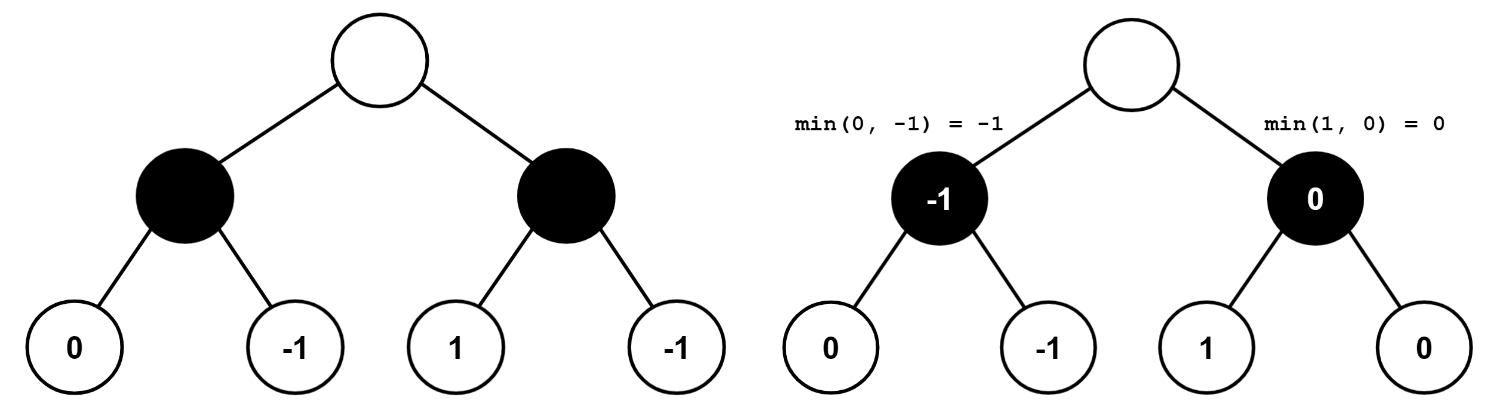
\includegraphics[scale=0.4]{img/minimax_step_0.png}
    \caption[Beispiel für die Auswahl eines Zuges mit dem Minimax-Algorithmus]{Beispiel für die Auswahl eines Zuges mit dem Minimax-Algorithmus \\ (eigene Anfertigung)}
\end{figure}

In diesem Fall gibt es zwei mögliche nächste Züge. Wichtig ist, dass nach jedem Zug der Spieler wechselt und der Algorithmus 
immer davon ausgehen muss, dass der Gegner den Zug mit dem höchsten Wert für ihn, also dem niedrigsten Wert für die KI wählt. 
Für das Beispiel heißt das, dass wenn der Gegner am Zug ist (schwarze Knoten), er den niedrigsten Wert, hier also -1 wählt. 
Das Gleiche gilt für den zweiten schwarzen Knoten, wo der Wert 0 ausgewählt wird.

Im nächsten Schritt ist die KI wieder am Zug, also wird diesmal der maximale Wert der möglichen Züge bestimmt. Konkret heißt das, 
dass wenn der rechte Zug gewählt wird, im schlechtesten Fall ein Unentschieden und beim linken Zug eine Niederlage erzielt werden kann. 
Um die Niederlage abzuwenden wird der rechte Zug und damit der höhere Wert gewählt.\autocite[Vgl.][S. 2]{GlennStrong.2011}

\begin{figure}[H]
    \centering
    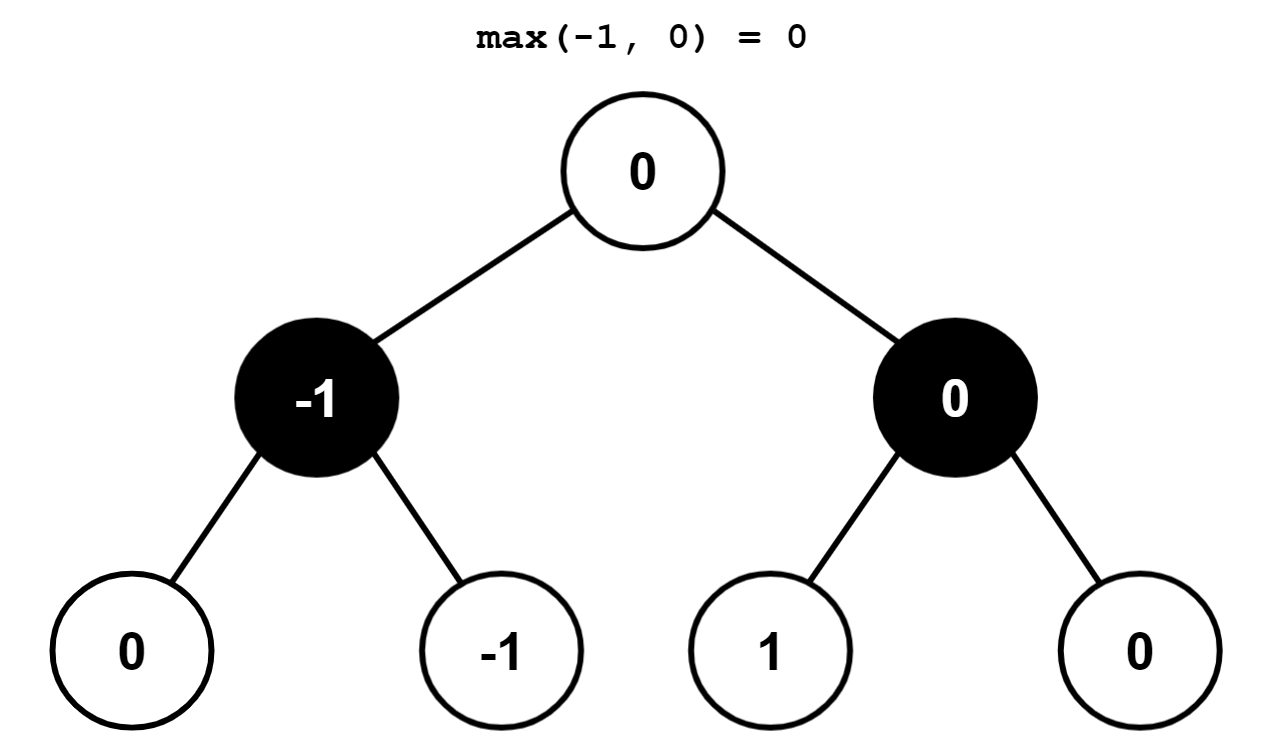
\includegraphics[scale=0.25]{img/minimax_step_1.png}
    \caption[Auswahl des finalen Spielzuges]{Auswahl des finalen Spielzuges (eigene Anfertigung)}
\end{figure}

Anzumerken ist, dass bei jedem Aufruf der Funktion \code{value} alle weiteren möglichen Spielzüge berechnet werden. 
Beim Spiel Tic-Tac-Toe kann es vorkommen, dass mehrere unterschiedliche Spielverläufe im selben Zustand enden. 
Für die Funktion \code{value} heißt das, dass sie mehrfach mit denselben Parametern aufgerufen wird und dadurch 
Rechenleistung verschwendet wird. Um redundante Funktionsaufrufe zu vermeiden wird das Prinzip der Memoisierung 
verwendet. D. h. es wird z. B. ein Dictionary verwendet, um bereits berechnete Ergebnisse zu speichern. Wird nun 
die Funktion \code{value} aufgerufen, wird erst geprüft, ob für die Parameter bereits ein Eintrag im Dictionary 
vorhanden ist. Ist dies der Fall, wird dieser Wert zurückgegeben und es findet keine Berechnung statt. Ist dem nicht 
so, wird ein neuer Eintrag im Dictionary angelegt.

\section{Unterschiede zwischen den Programmiersprachen Java und Python}
\label{chap:unterschiede_python_java}
Neben den in Kapitel \ref{chap:implementierungen} gezeigten Unterschieden bei der Implementierung, können weitere Unterschiede 
bei der Performance durch die unterschiedlichen Funktionsweisen und Eigenschaften der beiden Sprachen entstehen.

\subsection{Performanceunterschiede}
Ähnlich wie Java nutzt auch Python eine virtuelle Maschine, um Plattformunabhängigkeit umzusetzen. Dabei wird der Code 
zunächst in den jeweiligen Bytecode der virtuellen Maschine übersetzt und anschließend mit Hilfe eines Interpreters während 
der Laufzeit in Maschinencode übersetzt. Kompilierte Sprachen werden vor dem Ausführen vollständig in Maschinensprache übersetzt, den der 
jeweilige Prozessor anschließend ausführt. Beim Interpretieren von Code, werden einzelne Anweisungen zur Laufzeit schrittweise 
in Maschinencode übersetzt. Diese Vorgehensweise bietet den Vorteil, dass das Debugging einfacher ist, da hier Anweisungen 
einzeln übersetzt und ausgeführt werden und somit Fehler leichter im Code lokalisiert werden können. Der Nachteil ist, dass 
interpretieren deutlich langsamer ist als kompilieren, da der Code während der Laufzeit übersetzt werden muss. Da Java Programme 
in der Java Virtual Machine (JVM) ausgeführt werden, wird der Code zunächst in plattformunabhängigen Java Bytecode übersetzt. 
Der Java Bytecode muss anschließend in Maschinencode übersetzt werden. Dies erfolgt einerseits durch Interpretieren des Codes 
zur Laufzeit. Um die Performance zu verbessern wird der Interpretierungsprozess von einem Just in Time (JIT) Compiler unterstützt, 
der gegebenenfalls Java-Bytecodesequenzen in Maschinencode übersetzt, was die Laufzeit deutlich reduziert.\autocite[Vgl.][]{Aboullaite.31.8.2017}
Python nutzt hingegen standardmäßig keinen JIT-Compiler. Das hat zur Folge, dass auch keine JIT-Optimierung zur Laufzeit stattfindet 
und damit die Laufzeit höher ausfällt als bei Java.\autocite[Vgl.][]{Shaw.16.7.2018}

Ein weiterer wichtiger Aspekt, der die Performance von Python stark beeinflusst, ist die dynamische Typisierung von Variablen. 
Während man Objekten in Java immer einen festen Datentyp zuweisen muss, ist dies in Python nicht nötig. So können Variablen on the 
fly den Typ wechseln, was das Programmieren in vielen Fällen deutlich vereinfacht. Für die Performance ist dynamische Typisierung 
nicht förderlich. Um logische Operationen durchführen zu können, müssen Objekte intern typisiert werden, was Python komplett übernimmt. 
Da dieser Mehraufwand in Java nicht notwendig ist, ist Java in vielen Fällen deutlich performanter als Python.\autocite[Vgl.][]{Shaw.16.7.2018}


\subsection{Memory Management und Garbage Collection}
Während Python oft als unperformant wahrgenommen wird, konnte Python beim Arbeitsspeicherverbrauch im Vergleich 
zu Java punkten. Dies kann vor allem durch Unterschiede beim Speichermanagement der beiden Sprachen erklärt werden. 

Arbeitsspeicher wird in Python über einen Heap, der intern verwaltet wird. Wird also Arbeitsspeicher benötigt, 
wird dieser durch das Memory-Management vom Betriebssystem angefordert. Objekte bleiben nur so lange im Speicher 
wie sie benötigt werden. Python nutzt das sogenannte Reference Counting, um Objekte zu speichern.

\begin{lstlisting}[caption={Codebeispiel zur Verwaltung von Objekten in Python}]
    a = 9
    b = 9
    c = 11
\end{lstlisting}

In diesem Beispiel wird der Wert 9 als Objekt im Speicher erstellt und Variable \code{a} zugewiesen. Da 
Das Objekt mit dem Wert 9 schon existiert, wir Variable {b} als weitere Referenz hinzugefügt. Für Variable 
\code{c} heißt das, dass ein Objekt mit dem Wert 11 angelegt werden muss und \code{c} als Referenz hinterlegt wird. 
Beträgt die Anzahl der Referenzen eines Objekts Null, so wird es aus dem Speicher entfernt. Die Referenzen 
werden zyklisch vom Garbage Collector überprüft und Objekte ohne Referenzen entfernt.\autocite[Vgl.][]{PabloGalindoSalgado.2021} 
Reference Counting hat den Vorteil, dass nicht genutzter Speicher sehr schnell erkannt wird. Allerdings entsteht durch das Zählen 
der Referenzen ein gewisser Overhead, der im Vergleich zu anderen Garbage Collecting Verfahren aber eher gering ausfällt, 
zudem gibt es Sonderfälle, bei denen dieses Verfahren nicht zuverlässig funktioniert und deshalb zusätzlicher Aufwand 
betrieben werden muss, um den Speicher freizuhalten.

Im Gegensatz zu Python können für die meisten Objekte keine mehrfachen Referenzen vergeben werden. Stattdessen wird für jedes 
Objekt Speicher allokiert. Für das Codebeispiel heißt das, dass für alle drei Variablen zunächst 4 Bytes zum Speichern der 
der Integerwerte angefordert, die Referenz zur Variable hinterlegt und schließlich der Wert gespeichert wird. Hierbei spielt 
es keine Rolle, ob ein Wert mehrfach vorkommt, er wird trotzdem separat gespeichert. Eine Ausnahme bilden hierbei Strings. 
Diese werden ähnlich wie in Python mehrfach referenziert werden. Um nicht genutzten Speicher wieder freizugeben, wird der Heap 
regelmäßig auf Objekte geprüft, die nicht mehr verwendet werden. Der Prozess ist dabei in zwei Phasen eingeteilt. In der Mark-Phase 
werden noch relevante Objekte markiert. In der Sweep-Phase, werden die Lücken zwischen diesen Objekten dokumentiert und schließlich 
freigegeben.\autocite[Vgl.][]{OracleGC.2021}

\section{These zum Performanceunterschied}

Die in Kapitel \ref{chap:unterschiede_python_java} Unterschiede von Java und Python zeigen, dass Java durch den in der JVM integrierten 
JIT-Compiler und die statische Typisierung in den meisten Fällen eine bessere Performance aufweist, als Python. 
Dynamische Typisierung hat den Vorteil, dass sie für den Entwickler einfacher in der Handhabung ist. Diese macht allerdings 
Codeoptimierung hinsichtlich der verwendeten Datentypen unmöglich, weshalb trotz Memoisierung eine bessere Laufzeit von 
Java zu erwarten ist.